\documentclass[a4paper]{article}

\usepackage[a4paper,top=2cm,bottom=2cm,left=3cm,right=3cm,marginparwidth=1.75cm]{geometry}
\usepackage[utf8]{inputenc}
\usepackage[T1]{fontenc}
\usepackage{textcomp}
\usepackage[ngerman]{babel}
\usepackage{amsmath, amssymb, nccmath}
\usepackage{accents}


\usepackage{multirow}
\usepackage{fancyhdr}
\usepackage{lastpage}

% figure support
\usepackage{import}
\usepackage{xifthen}
\pdfminorversion=7
\usepackage{pdfpages}
\usepackage{transparent}
\newcommand{\incfig}[1]{%
    \def\svgwidth{\columnwidth}
    \import{./figures/}{#1.pdf_tex}
}

\pdfsuppresswarningpagegroup=1

\title{Protokoll zur ersten Laborübung\\Messtechnik Labor 376.091}
\author{DINC Atilla (11917652)}

\begin{document}
\newcommand{\unit}[1]{\ensuremath{\, \mathrm{#1}}} % Einheiten in Math-Moder richtig formatieren
% --------------------- HEADER ---------------------
\pagestyle{fancy}
% --------------------- FOOTER ---------------------
\fancyfoot[L]{Wintersemester 2023}
\fancyfoot[C]{\textbf{\thepage /\pageref{LastPage}}}
\renewcommand{\footrulewidth}{0.4pt}

\normalsize
\maketitle
\tableofcontents

\begin{center}
	\begin{tabular}{|c| c| c| c| c|}
		\hline
		\multicolumn{5}{|c|}{\textbf{Geräteliste}}                                                                                        \\
		\hline

		Bezeichnung              & Gerätebeschreibung                                         & Messgrößen & Inventarnummer & Bemerkungen \\
		\hline
		MM0                      & Agilent Digitalmultimeter True RMS                                  & -          & U1232A         & -           \\
		MM1                      & Digitalmultimeter                                          & -          & \#11            & -           \\
		MM2                      & Digitalmultimeter                                          & -          & \#7             & -           \\
		%\multirow{2}{*}{OZ1}     &
		%\multirow{2}{*}{
		%\begin{tabular}[c]
		%		Digitalspeicheroszilloskop DSO-x2002A \\
		%		MMSR
		%	\end{tabular}
		%}& \multirow{2}{*}{-} & \multirow{2}{*}{C0404-5} & \multirow{2}{*}{-}  \\
		                         &                                                            &            &                &             \\
		NG1                      & Netzgerät 2-Channel $\pm10\unit{mV}$                       & -   & CD0404-6       & -           \\
		FG1                      & Funktionsgenerator                                         & -    & SDG1025        & -           \\
		\hline
		\hline
		\multicolumn{5}{|c|}{\textbf{Zubehörliste}}                                                                                       \\
		\hline

		Bezeichnung              & Zubehörbeschreibung                                        & Messgrößen & Inventarnummer & Bemerkungen \\
		\hline
		K1                       & Tastkopf (10:1) 100\unit{MHz} 10\unit{M\Omega} 15\unit{pf} & -          & -              & rot         \\
		K2                       & Tastkopf (10:1) 150\unit{MHz} 10\unit{M\Omega} 15\unit{pf} & -          & -              & grau        \\
		K3                       & Tastkopf (10:1) 150\unit{MHz} 10\unit{M\Omega} 15\unit{pf} & -          & -              & rosa        \\
		\hline
	\end{tabular}
\end{center}
\newpage
% ~~~~~~~~~~~~~~~~~~~~~~~~~~~~ Start of the document ~~~~~~~~~~~~~~~~~~~~~~~~~~~~

\section{Einleitung}

\section{Messungen mit dem Digitalmultimeter}
\subsection{Spannungsmessung}
Zur Spannungsmessung wird der Spannungseingang des Multimeters parallel zur Messgröße
geschaltet, daher ist ein möglichst hoher Innenwiderstand $R_{i}$ erwünscht. Zur
Bestimmung dieses Innenwiderstands $R_{i}$ sollte eine Serienschaltung mit einem 
relativ hochohmigen bekannten Widerstand aufgebaut und der Spannungsabfall am Multimeter
von diesem abgelesen werden.\newline
Weiters sollte der Einfluss des Multimeters auf die Schaltung gemessen werden,
indem der Spannungseingang eines Multimeters des gleichen Models parallel zum 
Multimeter angeschlossen wird. \newline
Zuletzt sollte eine Messbereichserweiterung durchgeführt werden, indem ein
Serienwiderstand bekannter Größe in den Strompfad verbaut und der 
Spannungsabfall gemessen wird gemessen wird.

\subsubsection{Messaufbau und Messdurchführung}
\subsubsection*{Bestimmung des Innenwiderstands}
Die eingestellte Spannung des Netzgerätes FG1 wurde mit dem Multimeter MM0 
geprüft bevor sie mit der Schaltung belastet wurde. Der Serienwiderstand R1 wurde
mit dem Multimeter MM0 bestimmt.
Im Anschluss wurde die Schaltung wie in Abb. \ref{fig:1a_RiVM} angeschlossen.
Die angezeigte Spannung am Multimeter MM1 wurde abgelesen und die Eingangsspannung
wurde erneut gemessen. Weder die Eingangsspannung, noch die Spannung am Multimeter
MM1 haben sich geändert. Somit wurde sichergestellt, dass sowohl Innenwiderstand
des Netzgerätes, als auch jegliche Kontaktwiderstände in der Schaltung
vernachlässigbar klein für unsere Messungen waren.\newline
Der Kontrollprozess wurde vor allen folgenden Messungen durchgeführt, um die
Eingangsspannung möglichst genau zu bestimmen.
\begin{figure}[h]
    \centering
    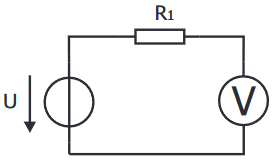
\includegraphics[width=0.4\textwidth]{schematics/1a_RiVM.png}
    \caption{Schaltung zur Bestimmung des Multimeter-Innenwiderstands}
    \label{fig:1a_RiVM}
\end{figure}

\subsubsection*{Bestimmung des Einflusses}
Für diese Messung wurde die Eingangsspannung $U_{q}$ wie zuvor gemessen.
Als Widerstand $R_{M}$ wurde der gleiche Widerstand wie zuvor verwendet und auch
und auch das Multimeter MM1 wurde nicht gewechselt, somit konnte die vorherige
Schaltung beibehalten und wie in Abbildung \ref{fig:1b_EinflussVM} erweitert werden.
Die Spannungen an den Multimetern wurden zunächst mit nur einem Multimeter MM1
und danach mit beiden Multimetern MM1 und MM2 abgelesen.
\begin{figure}[h]
    \centering
    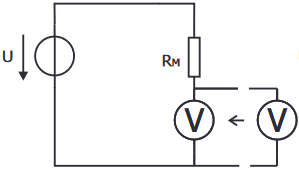
\includegraphics[width=0.4\textwidth]{schematics/1b_EinflussVM.png}
    \caption{Schaltung zur Bestimmung des Einflusses}
    \label{fig:1b_EinflussVM}
\end{figure}

\subsubsection*{Messbereichserweiterung}
Zur Messbereichserweiterung wurde die Schaltung wie in Abb. \ref{fig:1c_MB-ErweiterungVM}
aufgebaut. Dabei wurde der Widerstand $R_{M}$ aus der vorherigen Schaltung
und zur Messbereichserweiterung verwendet. Die zu messenden Spannungen in dieser
Schaltung ist die Eingangsspannung $U_{q}$ und sie soll in etwa halbiert werden, indem
die Widerstände mit $R_{M}\approx R_{V}$ auch in etwa gleich groß gewählt werden.
\begin{figure}[h]
    \centering
    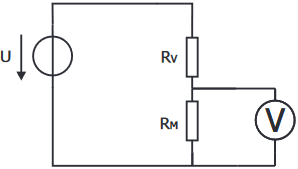
\includegraphics[width=0.4\textwidth]{schematics/1c_MessbereichserweiterungVM.png}
    \caption{Schaltung zur Messbereichserweiterung eines Voltmeters}
    \label{fig:1c_MB-ErweiterungVM}
\end{figure}

\subsubsection{Messergebnisse}
\subsubsection*{\textbf{Bestimmung des Innenwiderstands}}
Die Schaltung wurde mit einer gemessenen Eingangsspannung $U_{q}=9,92\unit{V}$ und einem
gemessenen Widerstand $R_{1}=98,9 \unit{k\Omega}$ aufgebaut. Weiters wurde am
Multimeter MM2 die Spannung $U_{V}=9,84\unit{V}$ gemessen. Mithilfe der Formel
für den Spannungsteiler kann die Gleichung
\[ U_{V}=U_{q} \frac{R_{i}}{R_{1}+R_{i}} = U_{q} \frac{1}{1 + \frac{R_{1}}{R_{i}}}\]
aufgestellt werden, woraus sich direkt durch Umformung
\[ R_{i}=\frac{R_{1}}{\frac{U_{q}}{U_{v}}-1}\approx 12,1647 \unit{M\Omega} \]
ergibt.

\subsubsection*{\textbf{Bestimmung des Einflusses}}
Auch bei dieser Messung wurde mit dem Handmultimeter MM0 eine Eingangsspannung
$U_{q}=9,92V$ verifiziert. Der Widerstand wurde wieder zu $R_{1}=98,9 \unit{k\Omega}$ gemessen.
Damit wurden die Messergebnisse wie in Tabelle \ref{tab:1b_Ergebnisse} aufgenommen.
Der Einfluss ergibt sich zur relativen Abweichung
\[ \Delta u_\text{MM1[\%]} =
        \frac{9,73\unit{V} - 9,84\unit{V}}{9,84\unit{V}} \cdot 100
    \approx -1,12\% .\]
\begin{table}[h]
    \centering
    \caption{Messergebnisse zum Einfluss eines Voltmeters}
    \label{tab:1b_Ergebnisse}
    \begin{tabular}{|c|c|c|}
        \hline
         & $U_{\text{MM1}}$&  $U_{\text{MM2}}$\\ 
        \hline
        vorher &$9,84\unit{V}$& $-$\\
        \hline
        nachher &$9,73\unit{V}$& $9,71\unit{V}$\\
        \hline
    \end{tabular}
\end{table}

\subsubsection*{Messbereichserweiterung}
Auch hier wurden die Eingangsspannung $U_{q}=9,92\unit{V}$ sowie der Widerstand 
$R_{M}=98,9\unit{k\Omega}$ gemessen. Weiters wurde der Widerstand
$R_{V}=99,5\unit{k\Omega}$ gemessen. Mit dem gemessenen Spannungsabfall
$U_{M}=4,93\unit{V}$ kann die Eingangsspannung $U_{q}$ über das messbereichserweiterte
Multimeter gemessen werden.
Aus der Maschengleichung folgt direkt
\[ U_{q}=R_{V}I+U_{M} = R_{V} \bigg(\frac{U_{M}}{R_{M}} + \frac{U_{M}}{R_{i}}\bigg) + U_{M} \]
\[ \implies U_{q}=U_{M}\bigg(1+\frac{R_{V}}{R_{M}} + \frac{R_{V}}{R_{i}} \bigg)
\approx 9,93 \unit{V}\]
\[ \implies f_{ME}=\frac{U_{q}}{U_{M}}\approx  2,0142\]


\subsection{Strommessung}
Ähnlich zur Messung mit einem Voltmeter wird auch bei einer Strommessung die
Schaltung durch das Amperemeter belastet. Da ein Amperemeter seriell zum
stromdurchflossenen Bauteil verschaltet wird, muss der Innenwiderstand möglichst
klein sein, um einen möglichst keinen Spannungsabfall zu verursachen.
Weiters kann der Messbereich eines Amperemeters erweitert werden, indem der
"überschüssige" Strom über einen parallelen Widerstand abgeführt wird.\newline
In diesem Abschnitt sollten analoge Schritte wie bei der Spannungsmessung durchgeführt werden: 
der Innenwiderstand $R_{i}$ und der Einfluss auf die Schaltung sollen bestimmt 
und eine Messbereichserweiterung sollte durchgeführt werden.

\subsubsection{Messaufbau und Messdurchführung}
\subsubsection*{Bestimmung des Innenwiderstands}

\begin{figure}[h]
    \centering
    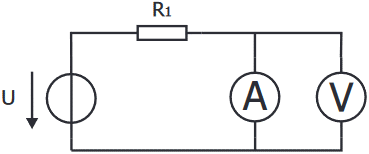
\includegraphics[width=0.4\textwidth]{schematics/2a_RiAM.png}
    \caption{Schaltung zur Bestimmung des Innenwiderstands}
    \label{fig:2a_RiAM}
\end{figure}

\subsubsection*{Bestimmung des Einflusses}

\begin{figure}[h]
    \centering
    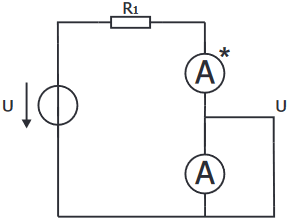
\includegraphics[width=0.4\textwidth]{schematics/2b_EinflussAM.png}
    \caption{Schaltung zur Bestimmung des Einflusses}
    \label{fig:2b_EinflussAM}
\end{figure}

\subsubsection*{Messbereichserweiterung}

\begin{figure}[h]
    \centering
    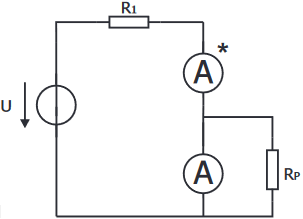
\includegraphics[width=0.4\textwidth]{schematics/2c_MessbereichserweiterungAM.png}
    \caption{Schaltung zur Messbereichserweiterung}
    \label{fig:2c_MB-ErweiterungAM}
\end{figure}

\subsubsection{Messergebnisse}
\subsubsection*{Bestimmung des Innenwiderstands}
Die tatsächliche Größe des Vorwiderstands wurde mit dem Handmultimeter vermessen
und betrug $R_{1}=4,68\unit{k\Omega}$.
Nachdem ein Anzeigestrom am Amperemeter von $I_{A}=500\unit{µA}$ eingestellt wurde,
stellten sich eine Gesamtspannung $U_{q}=2,382\unit{mV}$ und eine Spannung am
Amperemeter $U_{A}=50,5 \unit{mV}$ ein.\newline
Es lässt sich direkt der Innenwiderstand berechnen zu
\[ R_{i}= \frac{U_{A}}{I_{A}}= 101\unit{\Omega} ,\]
dieses Ergebnis ist für den niedrigen Strombereich des Multimeters sinnvoll.

\subsubsection*{Bestimmung des Einflusses}
Wie auch zuvor wurden Vorwiderstand $R_{1}=4,68\unit{V}$ sowie
Gesamtspannung $U_{q}=2,413V$ vermessen. Nach der Messung wurden die
Messergebnisse aus Tabelle \ref{tab:2b_EinflussAM} aufgenommen.
\[ f_{A}=\frac{490\unit{\mu A}}{500\unit{\mu A}} =0,98\]
\begin{table}[h]
    \centering
    \caption{Messergebnisse zum Einfluss des Amperemeters}
    \label{tab:2b_EinflussAM}
    \begin{tabular}{|c|c|c|}
        \hline
     & $I_{A}$  & $I_{A*}$\\ 
     \hline
        vorher & - & $500\unit{\mu A}$ \\
        \hline
        nachher & $495\unit{\mu A}$ & $490\unit{\mu A}$\\
     \hline
    \end{tabular}
\end{table}

\subsubsection*{Messbereichserweiterung}
Der gemessene Parallelwiderstand betrug $R_{P}=9,9\unit{k\Omega}$.
Mit diesem Widerstand wurde die Zweigströme $I_{A*}=500\unit{\mu A}$ und
$I_{A}=499\unit{\mu A}$ gemessen.
\[ \implies f_{ME}=\frac{I_{A*}}{I_{A}}\approx 1,002 \]
Diese Werte haben sich bei einer Versorgungsspannung $U_{q}=2,458\unit{V}$ eingestellt.

\section{Messungen mit dem Oszilloskop}
\subsection{Tastkopf}
\subsection{AC-Spannungsmessung}
\subsection{RMS im Detail}
\subsection{Amplitudenauflösung}
\subsection{Dynamik}


\end{document}
